\documentclass[tikz, border=5mm, a4paper]{book}

\usepackage{geometry}
\usepackage{amsmath}
\usepackage{hyperref}
\usepackage{blindtext}
\usepackage{graphicx}
\usepackage{listings}%For code do \begin{lstlisting}
\usepackage{color}
\usepackage{tikz-cd}
\usepackage{tikz}
\usepackage{float}
\usepackage{glossaries}
\usepackage{fancyhdr}
\usepackage{cleveref}
\usepackage{epigraph}
\usepackage{bytefield}
\usepackage{etoolbox}


\usetikzlibrary{arrows, arrows.meta, backgrounds, shapes, automata, petri, positioning, calc, chains, decorations.pathmorphing, fit, decorations.pathreplacing}


\definecolor{dkgreen}{rgb}{0,0.6,0}
\definecolor{gray}{rgb}{0.5,0.5,0.5}
\definecolor{mauve}{rgb}{0.58,0,0.82}
\definecolor{backcolour}{rgb}{0.95,0.95,0.92}

\lstset{frame=tb,
  aboveskip=3mm,
  belowskip=3mm,
  showstringspaces=false,
  columns=flexible,
  basicstyle={\small\ttfamily},
  numbers=left,
  numberstyle=\tiny\color{gray},
  keywordstyle=\color{blue},
  commentstyle=\color{dkgreen},
  stringstyle=\color{mauve},
  breaklines=true,
  breakatwhitespace=true,
  tabsize=3
}

\bibliographystyle{plain}

\makeatletter
\patchcmd{\chapter}{\if@openright\cleardoublepage\else\clearpage\fi}{}{}{}
\makeatother

\DeclareRobustCommand{\comment}[1]{
    {\color{orange}\emph{#1}}
}


{
\newglossaryentry{DSL}{name={\textbf{Domain Specific Languages}},description={
        A language(i.e, not just a library) with abstractions targeted at a specific problem domain.
        \begin{itemize}
            \item \textit{External DSL} - A DSL is defined as a separate programming language.
            \item \textit{Internal/Embedded DSL} - A DSL is defined as a language-like interface to a library.
        \end{itemize} 
    }}
\newglossaryentry{GPL}{name={\textbf{General Purpose Languages}},description={
    A language suited for a wide variety of problems and situations but lacks specialized features to deal with specific programs like a DSL.
}}
\newglossaryentry{syntax}{name={\textbf{Syntax}},description={Syntax refers to the rules that define the structure of a language. 
                                                    Syntax in computer programming means the rules that control the structure of the symbols, 
                                                    punctuation, and words of a programming language.}}

\newglossaryentry{semantics}{name={\textbf{Semantics}},description={The semantics of a program concerns the meaning of the program. i.e. what it does. 
                                                            It can take many forms, sometimes we're only interested in the result of the program.
                                                            Other cases concern the steps taken by the program to reach the said output.}}
\newglossaryentry{interpreter}{name={\textbf{Interpreter}},description={An interpreter is a program that directly executes instructions written in a programming language.}}
\newglossaryentry{compiler}{name={\textbf{Compiler}},description={A compiler is a program that translates computer code(\textit{the source language}) into another language(\textit{the target language})
                                                                Compilers usually convert some high-level language to some lower-level language.}}
\newglossaryentry{AST}{name={\textbf{Abstract Syntax Tree}},description={An Abstract Syntax Tree(AST) is a tree representation of the syntactic structure of our program. 
                                                                Can be represented by using trees or terms, and described by an algebraic data type or regular tree grammar.}}
\newglossaryentry{meta-programming}{name={\textbf{Meta-Programming}},description={Metaprogramming is a programming technique in which computer programs treat other programs as their data. 
                                        It means that a program can be designed to read, generate, analyze, or transform other programs, and even modify itself while running.}}
\newglossaryentry{BTL}{name={\textbf{Basic Typed Language}},description={Simple language with a few types and expressions on those types }}
\newglossaryentry{BIPL}{name={\textbf{Basic Imperative Programing Language}},description={An extension of BTL, but with statements and control flow.}}
\newglossaryentry{expression}{name={\textbf{Expression}},description={An expression is a syntactic construct that can be evaluated in order to obtain its value. The resulting value is usually one of the program's types.}}
\newglossaryentry{wellformed}{name={\textbf{Wellformed}},description={Wellformedness is when a program is following all the rules. smileemoji}}
\newglossaryentry{store}{name={\textbf{Store}},description={Program memory, byte/value array, grows upwards.}}
\newglossaryentry{env}{name={\textbf{Enviroment}},description={Map describing where things are located in the \gls{store}. Kinda like a phonebook}}
\newglossaryentry{scope}{name={\textbf{Scope}},description={A collection of identifier bindings . i.e. what's captured by the environment at some point in the code.}}
\newglossaryentry{param}{name={\textbf{Parameter}},description={A parameter is a local variable that is initialized with the arguments. Also often contains how those args are to be treated.}}
\newglossaryentry{local var}{name={\textbf{Local Variable}},description={A local variable is a variable that only exists within a limited scope.}}
\newglossaryentry{stackframe}{name={\textbf{Stackframe}},description={The stackframe is a snapshot of how the program environment looks at a certain point in time. 
                                                                        The stackframe saves things that could be changed by running the procedure and lets us restore the program
                                                                        to the previous state without all the changes made by the procedure.}}
\newglossaryentry{argument}{name={\textbf{Argument}},description={An argument is a value provided to the procedure when it is run. When the procedure is run the parameters of the procedure are initialized with its corresponding argument.}}
\newglossaryentry{copy sem}{name={\textbf{Copy Semantics}},description={Type of argument passing where the parameters are initialized with the value of the arguments}}
\newglossaryentry{ref sem}{name={\textbf{Reference Semantics}},description={Type of argument passing where the parameters point to the address as the argument.}}
\newglossaryentry{SLE}{name={\textbf{Software Language Engineering}},description={Software Language Engineering is the scientific field that researches language development, and maintenance of formal descriptions, and tooling of software lanugages}}
\newglossaryentry{BNF}{name={\textbf{Backus-Naur Form}},description={Formal notation for describing grammars. Used to describe the syntax of a language.}}
\newglossaryentry{Sum of Products}{name={\textbf{Sum of Products}},description={See chapter 1.3}}
\newglossaryentry{lexical analysis}{name={\textbf{Lexical Analysis}},description={Lexical analysis is the process of converting a sequence of characters into a sequence of tokens.}}}
\newglossaryentry{syntax analyzer}{name={\textbf{Syntax Analyzer}},description={Takes a stream of tokens and checks if it follows the rules of the grammar. Outputs a parse tree that is then assembled into an AST}}
\newglossaryentry{semantic analyzer}{name={\textbf{Semantic Analyzer}},description={Takes an AST and checks if it follows the rules of the language. Outputs a annotated AST}}
\makenoidxglossaries
\input{figures/jørn.tex}

\newcommand{\alg}[2]{[\![#1]\!]_{#2}}

\newcommand{\descbox}[2]{\parbox[c][3.8\baselineskip]{0.95\width}{%
    % facilitates the creation of memory maps. Start address at the bottom,
    % end address at the top.
    % syntax:
    % \memsection{end address}{start address}{height in lines}{text in box}
}}
\newcommand{\memsection}[4]{%
  % define the height of the memsection
  \bytefieldsetup{bitheight=#3\baselineskip}%
  \bitbox[]{10}{%
    \texttt{#1}% print end address
    \\
    % do some spacing
    \vspace{#3\baselineskip}
    \vspace{-2\baselineskip}
    \vspace{-#3pt}
    \texttt{#2}% print start address
  }%
  \bitbox{16}{#4}% print box with caption
}

%
\begin{document}

    \pagestyle{fancy}
    \fancyhead{}
    \rhead{\rightmark}
    \lhead{\leftmark}
    \fancyfoot{}
    \fancyfoot[LO,RE]{\thepage}
    
    %Frontpage 
    
\begin{titlepage}
    \begin{center}
        \vspace*{1cm}

        \huge
        \textbf{Book of Magne}

        \vspace{0.5cm}
        \LARGE
        INF222 Crashcourse 2022
            
        \vspace{1.5cm}

        \textbf{Sander Wiig}

        \vfill
        
        \Large
        INF222 Crashcourse for v2022.\\
        Some sections are adapted from Anya's INF225 notes and course material.
            
        \vspace{0.5cm}
    
        
\includegraphics[width=0.4\textwidth]{UiBlogoMN_gray_m_Eng.png}\\
        \Large
        Institute for Informatics\\
        University of Bergen\\
        Norway\\
        \today
            
    \end{center}
\end{titlepage}
\newpage
\tableofcontents
\newpage
    \newpage
    
    \tableofcontents
    \newpage
    
    \chapter*{Preface}
    The goal of this script is to provide an overview of the course INF222 at the University of Bergen.\\
    It is by no means a comprehensive guide to the course, but rather a supplement to the lectures and exercises.\\
    This was all written throughout a weekend and there is probably a whole lot wrong with the text and the code, so if you find any errors, please let me know by submitting a ticket or pull request on GitHub.\\
    The Glossary is especially lacking. Due to the time constraints, I was not able to update all terms in the glossary, so if you find a term that is not defined, or seems wrong, please let me know.\\
    
    \section*{Contributors}
    The following people have contributed in some way to this book:
    \begin{itemize}
        \item \textbf{Magne Haveraaen} for going over the course outline, and for teaching me what I know.
        \item \textbf{Anya Bagge} for her excellent INF225 notes, and for being a great teacher\cite{anya:2016}.
        \item \textbf{Jørn Lode} for his amazing figures that illustrate how states work.
        \item \textbf{Ralf Lämmel} for his book on Software Language Engineering, which much of this book is based on\cite{lammel:2018}.
        \item \textbf{} for proofreading, and verifying what I have written. 
    \end{itemize}

    \begin{figure*}[!h]
        \centering
        
\includegraphics[scale=0.3]{assets/qrcode.png}
        \caption{\url{https://github.com/Swi005/Book-of-Magne/tree/v2023}}
        \label{fig:qr}
    \end{figure*}

    \newpage
    \newpage
    
    \chapter{What is a language}
\section{What is a programming language}
    A programming language 
    \begin{itemize}
        \item is an artificial language(i.e made by us humans on purpose)
        \item used to tell machines what to do
    \end{itemize}
    More formally a programming language is a set of rules that converts some input, like strings, into instructions that the computer can follow.
    This is of course a very general description and it, therefore, follows that there are many different types of programming languages.
    IT therefore should come as little surprise that we group languages by features and properties. 
    \cite{anya:2016}

    \subsection*{Types of languages}
    There are many ways of grouping languages. They can be grouped by Purpose, typing, paradigm, Generality vs. Specificity, and many more.
    For now, we're going to group them by paradigm, and Generality vs. Specificity.

    \subsection*{Generality vs. Specificity}
    Languages are usually grouped into two categories when based on their specificity.
    \begin{itemize}
        \item DSL
        \item GPL
    \end{itemize}

    \Gls{DSL} are as the name suggests languages with a "specific" domain.\\
    DSLs usually have limited scope and use. Examples are JSON and SQL.     
    A Domain-Specific Language is a programming language with a higher level of abstraction optimized for a specific class of problems. 
    Optimized for a certain problem/domain. 
    DSLs can be further subdivided into external DSL(separate programming languages), and internal DLS(language-like interface as a library.)\\


    \Gls{GPL} however are more general and can be used to solve many different problems in many different situations.
    These languages have a wide array
    of uses and are usually what we think of when we hear the words programming language. Examples of GPLs are Java and Haskell.\\
    
    \begin{figure*}[!h]
        \begin{tabular}{|c|c|c|c|}
            \hline
            \textbf{Characteristic} &\textbf{DSL } &\textbf{GPL}\\
            \hline
            \textbf{Domain} & Small and well-defined domain & Generality, many use cases\\
            \hline
            \textbf{Size} &Small ASTs & Large ASTs, often user extensible\\
            \hline
            \textbf{Lifespan} &As long as their domain &years to decades\\
            \hline
            \textbf{Extensibility} &Usually not extensible by users & Provides mechanisms for extensibility\\
            \hline
        \end{tabular}%
        \caption{Some more comparisons between GPLs and DSLs\cite{lammel:2018}}
    \end{figure*}%

    \subsection*{Syntax and Semantics}
    All programming languages have two parts; the \gls{syntax}, and the \gls{semantics}.\\
    Syntax is the study of \textit{structure}, just as semantics is the study of \textit{meaning}. 
    Or in other words, the syntax tells us \textit{how} to write legal programs, and the semantics tells us \textit{what} those programs do. 

    \section{Meta Programming}
    One of the harder things in the course is \gls{meta-programming}. INF222 is usually the first time you've encountered meta-programming and it can be hard a hard concept to grasp. 
    Meta-programming is programming \textit{about} programming. More properly meta-programs treat other programs as data. When you see a data structure like \gls{BTL} or \gls{BIPL} in Haskell it
    represents a program.


    \section{Sum of products}
        You may have encountered the term \gls{Sum of Products}, lets's quickly run over why we use the terms \textit{sum} and \textit{product} 
        to describe the data types, and show some examples in both Haskell and Java.

        \subsection*{Haskell}
            \begin{lstlisting}[language=Haskell]
data SomeType = A Bool Bool Bool
                | B Bool
                | C
            \end{lstlisting}
            Here the type SomeType has 3 constructors, A, B, and C, where A takes 3 parameters, B takes one, and C zero. 
            The type of SomeType could be expressed algebraically as
            \begin{align*}
                \underbrace{(\text{Bool} \times \text{Bool} \times \text{Bool})}_{A} + \underbrace{\text{Bool}}_{B} + \underbrace{1}_{C}
            \end{align*}
            The Bool type can take on 2 different values
            ( False and True ), so the constructor
            can construct $2 * 2 * 2 = 8$ different values, since there are 8 different combinations you can
            make from 3 booleans (e.g. A True False False is one example). The constructor B can
            produce 2 different values, and C can only produce one (not zero!).
            Thus, the total numbers of values of type SomeType is $8 + 2 + 1 = 11$, as the data type
            is the sum of the three products we've just described.\\
            In short, a sum type denotes “one of” its constituent types (if your function takes SomeType
            as input, it will get either (A b1 b2 b3 ), (B b1) or C for some boolean values b1 . . .), while
            a product type denotes “all of” its constituent types (e.g. a value constructed with A will
            have all 3 booleans present.) Another way to express a product type in Haskell is with tuples,
            e.g.
            \begin{lstlisting}[language=Haskell]
type MyTriple = (Bool, Int, Char)
            \end{lstlisting}

            \subsection*{Java}
            In Java, we can model the same kind of data types using classes and inheritance. The instance
            variables of a class determine a “product” type, e.g.

            \begin{lstlisting}[language=Java]
class SomeClass {
    boolean a;
    boolean b;
    boolean c;
}
            \end{lstlisting}
    Similar to the constructor for A in the previous section, there are $2 * 2 * 2 = 8$ different
    values an object of class SomeClass can have. Add another boolean, and you get 16 different
    values. Technically, a variable of type SomeClass can take one 8 + 1 different values, since
    null is also a valid value for all object variables in Java, but sometimes we ignore this fact
    and tell the users of our functions to kindly not pass in null as an argument where we expect
    an actual object.
    Now, to get sum types, we might use class hierarchies in Java:

    \begin{figure}[!h]
        \centering
        \begin{lstlisting}[language=Java]
interface SomeType {}

class A implements SomeType {
    boolean a;
    boolean b;
    boolean c ;
}
class B implements SomeType {
    boolean a;
}
class C implements SomeType {
}
        \end{lstlisting}
    \end{figure}

    Now, an object of type SomeType can (ignoring null) take on $8 + 2 + 1$ different values,
    just like in the Haskell example above.

    \newpage
    
    \chapter{Anatomy of an Interpreter}
\label{sec:anatomy}
        
An \gls{interpreter} is a computer program that directly executes instructions written in a programming language.
This differs from a \glspl{compiler} which translates a program from one language to another(usually to a lower level one ex. C or ASM).\\
We usually divide the compiler/interpreter process into two categories, front end, and back end.
The front end is the part of the compiler/interpreter that takes the source code and converts it into some intermediate representation.
In compilers, this is usually some form of byte code or 3-word code, that can then be translated into the target language. 
This is not necessary for an interpreter where the intermediary representation is often in the form of an annotated AST.
The back end is the part of the compiler/interpreter that takes the intermediary representation and executes it(in the case of interpreters) or translates it back into code(compilers).\\

\section{Phases of an interpreter}
An interpreter is composed of several phases. \\
The front end consists of the lexical analyzer, the syntax analyzer, and the semantic analyzer.\\
The backend is the evaluator.\\
The \gls{lexical analysis} takes the actual characters that the code is made up of and divides it up into its lexical tokens(by the tokenizer) using the concrete syntax of the program\footnote{Not covered by this course, so you can safely ignore how this works.... \textit{for now!}}. 
Take for instance the following expression:
\\
\begin{equation*}
    (1+2)*13
\end{equation*}\\
\\
The lexical analyzer would divide this into the following tokens:
\texttt{["(", "1", "+", "2", ")", "*", "13"]}
\newpage
This list of tokens is then sent to the \gls{syntax analyzer}\\
The syntax analyzer takes the token list and builds a parse tree out of the tokens and the concrete syntax (fig.\ref{fig:parsetree}).
\begin{figure}[!h]
    \centering
    \begin{tikzcd}
        \node[] (e0) {"expr"};
        \node[below left = of e0] (e1) {"expr"};
        \node[below left = of e1] (e11) {"("};
        \node[below = of e1] (e12) {"expr"};
        \node[below right = of e1] (e13) {")"};
        \node[below left = of e12] (e121) {"number"};
        \node[below = of e121] (e1211) {"1"};
        \node[below = of e12] (e122) {"+"};
        \node[below right = of e12] (e123) {"number"};
        \node[below = of e123] (e1231) {"2"};
        \node[below = of e0] (e2) {"*"};
        \node[below right = of e0] (e3) {"number"};
        \node[below = of e3] (e31) {"13"};

        \draw (e0) edge (e1)
            (e0) edge (e2)
            (e0) edge (e3)
            (e1) edge (e11)
            (e1) edge (e12)
            (e1) edge (e13)
            (e12) edge (e121)
            (e12) edge (e122)
            (e12) edge (e123)
            (e121) edge (e1211)
            (e123) edge (e1231);

    \end{tikzcd}
    \caption{Parse tree}
    \label{fig:parsetree}
\end{figure}

The parse tree is then converted into an \gls{AST} by the abstract syntax rules (fig.\ref{fig:ast}).

\begin{figure}[!h]
    \centering
    \begin{tikzcd}
        \node[] (e0) {\texttt{Mult}};
        \node[below left = of e0] (e1) {\texttt{Add}};
        \node[below left = of e1] (e11) {\texttt{1}};
        \node[below right = of e1] (e12) {\texttt{2}};
        \node[below right = of e0] (e2) {\texttt{13}};

        \draw (e0) edge (e1)
            (e0) edge (e2)
            (e1) edge (e11)
            (e1) edge (e12);
    \end{tikzcd}
    \label{fig:ast}
    \caption{AST}
\end{figure}

The syntax analyzer builds a parse tree out of the tokens and the concrete syntax. 
This is then converted into an AST by the abstract syntax rules. 
Which is then handed over to the next part, the \gls{semantic analyzer}.
The AST is type-checked, checked for well-formedness, names are resolved, and types are inferred. The new AST, now with added information, is then given to the evaluator so that it can be evaluated and produce a result.
See Fig. \ref{fig:interpreterphases}.

\begin{figure}[ht]
    \centering
    \begin{minipage}{.5\textwidth}
        \centering
        \fbox{\centering
        \begin{tikzcd}
            \parbox{\textwidth}{}\arrow[d, "\text{character stream}"]\\
            \fbox{\parbox{10em}{\centering Lexical Analyzer}}\arrow[d, "\text{token stream}"]\\
            \fbox{\parbox{10em}{\centering Syntax Analyzer}}\arrow[d, "\text{syntax tree(AST)}"]\\
            \fbox{\parbox{10em}{\centering Semantic Analyzer}}\arrow[d,"\text{syntax tree(Annotated AST)}"]\\
            \fbox{\parbox{10em}{\centering Evaluator}}\arrow[d, "\text{result}"]\\
            \parbox{\textwidth}{}
        \end{tikzcd}}
        \caption{Phases of an interpreter}
        \label{fig:interpreterphases}
    \end{minipage}%
    \begin{minipage}{.5\textwidth}
        \centering
        \fbox{\centering
        \begin{tikzcd}
            \parbox{\textwidth}{}\arrow[d, "\text{character stream}"]\\
            \fbox{\parbox{10em}{\centering Lexical Analyzer}}\arrow[d, "\text{token stream}"]\\
            \fbox{\parbox{10em}{\centering Syntax Analyzer}}\arrow[d, "\text{syntax tree(AST)}"]\\
            \fbox{\parbox{10em}{\centering Semantic Analyzer}}\arrow[d,"\text{syntax tree(Annotated AST)}"]\\
            \fbox{\parbox{10em}{\centering Intermediate Code Generator}}\arrow[d, "\text{Intermediate representation}"]\\
            \fbox{\parbox{10em}{\centering Machine-Independent Code Optimization}}\arrow[d, "\text{Intermediate representation}"]\\
            \fbox{\parbox{10em}{\centering Code Generator}}\arrow[d, "\text{target machine code}"]\\
            \fbox{\parbox{10em}{\centering Machine-Dependent Code Optimization}}\arrow[d, "\text{target-machine code}"]\\
            \parbox{\textwidth}{}
        \end{tikzcd}}
        \caption{Phases of a "normal" compiler}
        \label{fig:compilerphases}
    \end{minipage}%
    \caption{Please appreciate the figures above, they were hard to make}
\end{figure}%
\newpage
\section{ASTs \& Static Analysis}
    \section{ASTs}
        An \gls{AST} is the tree representation of the syntactic structure of a program; The abstract syntax
        describes the structure of the abstract syntax tree - it can be defined using a
        regular tree grammar, or an algebraic data type or term (in Rascal, ML, Prolog,
        ...), or an object-oriented inheritance hierarchy of node classes (Java, C++, ...),
        or as an S-expression (in Lisp languages).
        The abstract syntax tree can be used as an internal representation in a language processor, 
        but it is not the only possible representation.\\
        An abstract syntax can be generated by a grammar in the following way:
        For every non-terminal type, there is a corresponding abstract syntax type.
        Each type has one constructor (or node type) corresponding to each production in the grammar, with one child for every symbol in the production that
        is not a literal token (e.g., punctuation, keywords, or spaces). If a constructor
        has only one child, of the same type, it can be removed (e.g., this would be
        the case for a parenthesis expression). You can do this process entirely based
        on the information contained in a parse tree. Translating a parse tree into a
        corresponding abstract syntax tree is called imploding the parse tree.
        Given an abstract syntax tree, it is possible to reconstruct a parse tree or program text, given the original grammar - though the resulting program may be
        slightly different in terms of spaces and punctuation. 
        \newpage
        This is called unparsing or
        pretty-printing (particularly if the output is nicely formatted). Parsing, imploding, pretty-printing, and then reparsing may not yield the exact same parse tree
        as the original tree, but it should still implode to the same abstract syntax tree (otherwise there is a bug in your toolchain!).

        Various phases in a language processor may change the abstract syntax
        tree, or use slightly different versions of the abstract syntax (e.g., after type
        checking, the nodes for variables include the type of the variable) - it is also
        possible to decorate or annotate the AST as processing proceeds. 
        This adds extra information to the nodes in the AST, without impacting the structure of the abstract syntax.
        Important abstract syntax design considerations are;
        \begin{itemize}
            \item Simplicity. Generally, your compiler tools will do a lot of work on AST,
            and the fewer different cases you have to worry about, the better. For
            For example, if the processing of overloaded functions and operators is the same (which it is to some degree in C++), you may want to have
            only one AST node type to cover both. Having a lot of unnecessary nodes
            in the tree can be annoying as well, and may make processing slower.
            \item Good correspondence with the constructs of the language.
            \item Availability of information during processing. Some information 
            can be computed from the tree (such as type information) and might be encoded directly in the tree (at least at later stages) for easy processing.
            \item Being end-user friendly or familiar to most programmers isn't an important consideration - the abstract syntax may be radically different from
            the surface concrete syntax if that helps the compiler writer.
        \end{itemize}

    \section{Static Analysis}
        \subsection{Type Checking}
        Programming language typing always falls into one or two categories; static, and dynamic typing. Static typing is when type checking happens at compile-time, 
        while dynamic typing happens during runtime. We will focus on static typing. 
        Statically typed languages typically have these properties.
        \begin{itemize}
            \item Variables and data structures must be declared before use.
            \item Variables and data structure fields can only hold values of the declared type.
            \item Operations(i.e functions, procedures, methods) and types must be declared.
            \item Declaring the exact types of variables and operations isn't always needed. Some languages use type inference (Discussed in 3.2.3).
        \end{itemize}

        What is a type checker and how does it work? 
        A type checker is a meta-program that checks that verifies that the type of some construct(lists, expressions, etc.) matches what's expected of it.
        For example, a type checker will check that the Plus \gls{expression} takes two Integers. This lets the type checker discover and report certain errors before the program runs. 
        To do this a type checker needs to know;
        \begin{itemize}
            \item How the language should look.
            \item The language types.
            \item Rules for assigning types to the constructs.
        \end{itemize}
        \subsubsection*{Let's do a practical example}
        Here's the abstract syntax for our Simple Typed Language or STL for short.
        \lstinputlisting[language=Haskell, firstline=2, lastline=11]{figures/code/typecheck.hs}
        Before we can continue we need to define the types that are allowed. We decide to use two types, Integers, and Booleans.
        \lstinputlisting[language=Haskell, firstline=12, lastline=12]{figures/code/typecheck.hs}
        
        Now to the meat of the exercise, the type checker itself.
        The usual way to do this in Haskell(and most other languages I've experienced) is to define a series of recursive functions, one for each
        expression/operand.
        \lstinputlisting[language=Haskell, firstline=14, lastline=14]{figures/code/typecheck.hs}
        
        I have found it easiest, to begin with, the cases that form the basic "building blocks" of a language, the literals. It is easy to know the type of Int Literals(Integer obviously), and Bool Literals(Boolean).
        \lstinputlisting[language=Haskell, firstline=15, lastline=16]{figures/code/typecheck.hs}
        
        After these "base" cases we add a case for Vars, this is slightly more complicated since the type is dependent on the list of var declarations, 
        so we need to check the VarDecl list.
        \lstinputlisting[language=Haskell, firstline=18, lastline=21]{figures/code/typecheck.hs}
        
        We use a pretty clever Haskell expression called "case". This lets us pattern match the result of the function call in lookup. 
        I strongly recommend that you all learn how to use these since they are extremely useful and I'll be using them liberally during this example.\\
        We now move on to the ops.
        \lstinputlisting[language=Haskell, firstline=23, lastline=48]{figures/code/typecheck.hs}
        
        These all more-or-less follow the same pattern \footnote{Maya made me use fancier words, apparently "pretty similar" isn't good enough.}.
        They all check that the arguments are of the correct type and return the operand type if so, if not they raise an error.
        Eq is the odd one out since it returns a boolean no matter what since it checks if two expressions are the same.\\
        The last case is the most complex. Choice tests a boolean condition and returns one of the two expressions depending on the value.
        The problem is that we don't know which branch will return. We have therefore decided both branches need to be of the same type.
        \lstinputlisting[language=Haskell, firstline=50, lastline=57]{figures/code/typecheck.hs}
           
        Here we begin by checking that the test evals to a boolean type, if so we check that both branches have the same type and return that type.
        Note that even though an evaluator would only evaluate one of the two branches, we still type-check them both.
        
        
        \subsection{Wellformedness}
            For a program to be \gls{wellformed} it needs to satisfy all the constraints(think rules) on it. This means that the program follows all the rules 
            for it like; 
            \begin{itemize}
                \item The program conforms to the AST.
                \item It is typed correctly
                \item All procedure calls/declarations are wellformed.
                \item and much more.
            \end{itemize}

            \newpage
            To check if a program is wellformed we usually implement a so-called constraint checker. These are pretty much just unit tests.
            The recipe for a constrain checker is as follows;
            \begin{itemize}
                \item \textbf{Negative test cases} - Designate one negative test case for each constraint that should be checked. 
                Ideally, each such test case should violate only one constraint.
                \item \textbf{Reporting} - Choose an approach to "reporting". The result of constraint violation may be communicated either through
                                        a boolean value, as a list of errors, or by throwing an exception.
                \item \textbf{Modularity} - Implement each constraint in a separate function, thereby allowing modularity and testing.
                \item \textbf{Testing} - The constraint violations must be correctly detected for the negative test cases. The positive test case must pass.
            \end{itemize}

    
    \newpage
    
    \chapter{Store, State, and Storage}

\section{State}
\label{sec:state}
\subsection{Store}
\label{subsec:store}
When running a program we often want to remember intermediary values or have variables. For us to do this we need some way of storing values.
To do this we create a \gls{store}. A store is very simply an array, usually containing either bytes or ValueTypes. 
The store is the program's memory(this is true in C). To access a value located at $i$ in our store we simply access the value at array index $i$.
Worth noting that the store is what we call the program heap and by tradition, it grows upwards. This means that new entries are stored at the highest available index in our store.
This is because the stack grows upwards and gives us the best possible use of the memory.

\subsection{Variables and Enviroment}
\label{subsec:vars}
We now have a place to store stuff, but how do we know where it is in the store? This is where \glspl{env} comes into play.\\
An environment is a map between variables and their location in the store. \\
\comment{Elaborate more about variables as name bindings.}
\section{Scoping}
\label{sec:scope}

Most variables are not visible to the entire program.
In previous courses, you have in all likelihood encountered global and local variables when programming.
Where global variables are variables that are visible to the entire program, and local variables are variables that are only visible to the method or function that they were declared in.

The term for where a variable is visible is called the \gls{scope} of a variable.
Variable scoping is useful because it lets us keep variables in different parts of our programs separate.
If you were to write a calculator it would be somewhat awkward if you could only use \texttt{x} and \texttt{y} once.

\newpage
Scope can also apply to more than just variables, and all declarations usually have scope.
Most languages generally use one of three classes of scoping, and these can have wildly different effects on a program's semantics:

\begin{itemize}
    \item \textbf{Runtime Scoping} - In Runtime Scoping the variable that is in scope is determined by the execution of the program and is the variable that was last seen.
                                    Runtime scoping makes no difference between declaration and usage.                           
                                    Variables are declared, initialized, and updated as the interpreter proceeds with the code. 
                                    Depending on the code's branching structure, a variable may or may not be declared.
                                    This means that a variable's scope is often the entire program.
                                    
    \item \textbf{Static Scoping} - In Static Scoping the variable that is in scope is determined by the structure of the program. 
                                    This means that the variable that is in scope is the variable that was declared in the closest enclosing scope.
                                    A variable's scope is often just the block where it was declared.
                                    Static scoping is easy to reason about and is the most common form of scoping used today.
    \item \textbf{Dynamic Scoping} - In dynamic scoping the scope of a variable is determined by the usage context, instead of its declaration.
                                    Dynamic scoping is often hard to reason about since a variable has to be reasoned about in every usage context.
                                    Dynamic scoping is therefore not used very often.                      
\end{itemize}

To better illustrate the differences let's take a look at an example!

\begin{figure}[!h]
    \centering
    \lstinputlisting[language=c]{figures/code/scoping/scoping.c}  
    \caption{Scoping Example}
    \label{fig:scoping}
\end{figure}

\subsection*{Runtime Scoping}
If we execute the program with runtime-scoping the program will return 20. 
This is because the variable \texttt{x} is first declared in line 3, but is then overridden in \texttt{g()} on line 5.
When we call \texttt{g()} on line 9, the variable \texttt{x} is set to 20, and this is then returned by \texttt{f()}.

\subsection*{Static Scoping}
If we execute the program with static scoping the program will return 10.
This is because the variable \texttt{x} is first declared on line 3, before being shadowed in \texttt{g()}, but because \texttt{x} is only 20 within \texttt{g()}, the \texttt{x} in \texttt{f()} is still the same as it was on line 3.

\subsection*{Dynamic Scoping}
The result of executing the program with dynamic scoping is 20 because the variable \texttt{x} is set to 20 in \texttt{g()} and \texttt{g()} calls \texttt{f()}.


\section{Data Structures in Memory}
\subsection{Arrays}
An array is a type of data structure that holds a fixed number of elements of the same type.
Arrays are usually stored in memory as a contiguous block of memory.
Arrays are usually indexed by integers.

\begin{figure*}[h]
    \begin{lstlisting}[language=c]
        int foo[5] = {1, 2, 3, 4, 5};
    \end{lstlisting}
    \caption{Array of Ints with 5 elements.}
\end{figure*}
In the code above we have an array consisting of 5 integers, we'll assume that addresses only use 1 byte of memory, and integers take up 4 bytes.
Figure \ref{fig:array1} shows how the array would be stored in memory.

\begin{figure}[H]
    \centering
    \begin{bytefield}{8}
        \begin{rightwordgroup}{\texttt{foo} is a pointer to the array at \texttt{0x00}}
            \memsection{0xff}{}{1}{\texttt{foo}}
        \end{rightwordgroup}\\
        \memsection{0xfe}{}{4}{...}\\
        \begin{rightwordgroup}{The actual array}
            \memsection{0x13}{}{4}{5}\\
            \memsection{0x0f}{}{4}{4}\\
            \memsection{0xb}{}{4}{3}\\
            \memsection{0x08}{}{4}{2}\\
            \memsection{0x04}{0x00}{4}{1}
        \end{rightwordgroup}
    \end{bytefield}
    \caption{\texttt{foo} in memory}
    \label{fig:array1}
\end{figure}


The array is stored as a contiguous block of memory, and the variable \texttt{foo} is a pointer on the stack that points to the start of the array.
To access the elements in the array we can use the pointer \texttt{foo} and add an offset to it.
The address for the $n'th$ element in an array is given by the following formula, where

\begin{equation*}
    \texttt{foo[n]} = \texttt{\&foo} + n * \texttt{sizeof(int)}
\end{equation*}
\begin{itemize}
    \item \texttt{\&foo} is the pointer to the array
    \item \texttt{n} is the index of the element we want to access
    \item \texttt{sizeof(int)} is the size of an integer in bytes
\end{itemize}


\subsection{Matrixes and Multidimensional Arrays}
Things get a little bit more complicated when dealing with multidimensional arrays, and the exact nature of how multidimensional arrays are stored in memory depends on the language.
There are two main ways of storing arrays of arrays.
First is to that each entry in the outer array is a pointer to the nested array.
This has a few problems,\\
the first is that the cpu needs to do an extra memory lookup to get the address of the nested array.
The second is that it becomes impossible for the compiler to make memory layout optimizations that would otherwise be possible.

The second way is to store the entire array as a contiguous block of memory.
This has the advantage that the cpu can do a single memory lookup to get the address of the nested array, and the compiler can make optimizations.
The disadvantage is that the memory layout is not as intuitive(See Figure \ref{fig:array2}).
\begin{figure}[!h]
    \begin{minipage}{.3\textwidth}
        \centering
        \begin{lstlisting}[language = c]
int bar[3][3] = [
        [1, 2, 3],//First Row
        [4, 5, 6],//Second Row
        [7, 8, 9] //Third Row
    ];
        \end{lstlisting}
    \end{minipage}%
    \begin{minipage}{.3\textwidth}
        \centering
        \begin{bytefield}{8}
            \memsection{0xfffff}{0x0020}{4}{\dots}\\
            \begin{rightwordgroup}{Third row}
                \memsection{}{0x20}{4}{9}\\
                \memsection{}{0x1c}{4}{8}\\
                \memsection{}{0x18}{4}{7}
            \end{rightwordgroup}\\
            \begin{rightwordgroup}{Second row}
                \memsection{}{0x14}{4}{6}\\
                \memsection{}{0x10}{4}{5}\\
                \memsection{}{0x0c}{4}{4}
            \end{rightwordgroup}\\
            \begin{rightwordgroup}{First row}
                \memsection{}{0x08}{4}{3}\\
                \memsection{}{0x04}{4}{2}\\
                \memsection{}{0x00}{4}{1}
            \end{rightwordgroup}
        \end{bytefield}
    \end{minipage}
    \caption{\texttt{bar} in memory with contiguous layout}
    \label{fig:array2}
\end{figure}

\newpage

\subsection{Records, Structs}
Records are a data structure that can hold multiple values of different types.
Records are also known as structs, tuples, or classes depending on the language.


\begin{figure}[!h]
    \centering
    \begin{lstlisting}[language=c]
struct foo {
    int x; //Offset 0
    bool y; //Offset 4
    double z;//Offset 5
};
    \end{lstlisting}
\end{figure}
\begin{align*}
    |\texttt{foo}| &= |\texttt{x}| + |\texttt{y}| + |\texttt{z}| \\
    &= 4 + 1 + 8 = 13
\end{align*}
\begin{figure}[!h]
    \centering
    \begin{bytefield}{8}
        \begin{rightwordgroup}{\texttt{foo} is a pointer to the struct at \texttt{0x00}}
            \memsection{0xff}{}{1}{\texttt{foo}}
        \end{rightwordgroup}\\
        \memsection{0xfe}{0x0a}{4}{...}\\
        \begin{rightwordgroup}{The actual struct}
            \memsection{}{0x05}{8}{z}\\
            \memsection{}{0x04}{1}{y}\\
            \memsection{}{0x00}{4}{x}
        \end{rightwordgroup}
    \end{bytefield}
    \caption{\texttt{foo} in memory}
    \label{fig:struct1}
\end{figure}

\newpage

\subsubsection{Arrays of Records}
Storing records in memory is very straight forwards, as with arrays, there are two main ways of storing arrays of records.
The first is the one used by Java, where each element of the array is really a pointer to a record thats stored somewhere else on the heap.\\

The other way is to store them as you would any other datatype, as a contiguous block of memory, with one record stored after the other.

To access a field in a record we can use the following formula, where
\begin{equation*}
    \texttt{arr[n].x} = \texttt{\&arr} + n *|\texttt{foo}|+|\texttt{offset(x)}|
\end{equation*}
where 
\begin{itemize}
    \item \texttt{arr} is the Array
    \item \texttt{n} is the index of the element we want to access
    \item \texttt{foo} is the struct or record
    \item \texttt{x} is the field we want to access
\end{itemize}
    \newpage
    
    
\subsection*{What is a Procedure}
\begin{frame}{\textbf{What is a Procedure}}
    \begin{itemize}
        \item Procedures are "programs within programs"
        \item Procedures have their own environment
    \end{itemize}
    \begin{alertblock}{Functions vs. Procedures}
        \begin{equation}
            \text{Functions} \neq \text{Procedures}
        \end{equation}
        Functions are expressions, procedures are statements.\\
        Very often same implementation.
    \end{alertblock}
\end{frame}

\subsection*{Anatomy of a procedure}
\begin{frame}{\textbf{Anatomy of a Procedure}}
    \begin{figure}
        \lstinputlisting[language=Pascal]{examples/anatomy.pipl}
    \end{figure}
    \begin{block}{Params}
        \begin{itemize}
            \item \textbf{OBS} - "read only"
            \item \textbf{UPD} - "read/write"
            \item \textbf{OUT} - "write only"
        \end{itemize}
    \end{block}
\end{frame}

\begin{frame}{\textbf{Declaration vs. Calling}}
    \begin{figure}
        \lstinputlisting[language=pascal, basicstyle=\ttfamily\tiny]{examples/ex1.pipl}
        \label{fig:ex1}
        \caption{Swap Procedure}
    \end{figure}
\end{frame}

\subsection*{Paramter Semantics}
\begin{frame}{\textbf{Parameter Semantics}}
    \Large
    Two types of parameter semantics:
    \begin{itemize}
        \item Reference semantics
        \item Copy semantics
    \end{itemize}
\end{frame}

\begin{frame}{\textbf{Reference Semantics}}
    \Large
    \begin{itemize}
        \item Parameters become aliased to arguments 
        \item Points to same memory address
        \item Unsafe, but sometimes useful
    \end{itemize}
\end{frame}
\begin{frame}{\textbf{Running a procedure with reference semantics}}
    \Large
    \begin{enumerate}[<+->]
        \item Get stackframe
        \item Wipe environment
        \item Add parameters to the environment with same address as arg
        \item run the procedure code
        \item restore the environment
    \end{enumerate}
\end{frame}
\begin{frame}{\textbf{Copy Semantics}}
    \Large
    \begin{itemize}
        \item Parameters are declared as variables and initialized with args' value
        \item Safer
        \item More intuitive behavior
        \item More complicated to implement
    \end{itemize}
\end{frame}

\begin{frame}{\textbf{Running a procedure with copy semantics}}
    
    \begin{enumerate}[<+->]
        \item Get stackframe
        \item Get values of args
        \item Wipe environment
        \item Add parameters to environment
        \item init those parameters with the arg values
        \item run the procedure code
        \item get the values of the parameters
        \item restore the environment
        \item copy the parameter values back to the args
    \end{enumerate}
\end{frame}


\subsection*{Reference semantics!}
\begin{frame}\textbf{{Reference semantics}}
    \lstinputlisting[language=Pascal]{examples/paramater semantics/copy/paramsem.pipl}
\end{frame}
\begin{frame}\textbf{{Reference semantics}}
    \lstinputlisting[language=Pascal]{examples/paramater semantics/copy/paramsem1.pipl}
\end{frame}
\begin{frame}\textbf{{Reference semantics}}
    \lstinputlisting[language=Pascal]{examples/paramater semantics/copy/paramsem2.pipl}
\end{frame}
\begin{frame}\textbf{{Reference semantics}}
    \lstinputlisting[language=Pascal]{examples/paramater semantics/copy/paramsem3.pipl}
\end{frame}

\subsection*{Example!}
\begin{frame}{\textbf{Swap example v2}}
    \lstinputlisting[language=Pascal]{examples/paramater semantics/paramsem.pipl}
\end{frame}

\subsection*{Copy semantics!}
\begin{frame}\textbf{{Copy semantics}}
    \lstinputlisting[language=Pascal]{examples/paramater semantics/reference/paramsem.pipl}
\end{frame}

\begin{frame}\textbf{{Copy semantics}}
    \lstinputlisting[language=Pascal]{examples/paramater semantics/reference/paramsem1.pipl}
\end{frame}
\begin{frame}\textbf{{Copy semantics}}
    \lstinputlisting[language=Pascal]{examples/paramater semantics/reference/paramsem2.pipl}
\end{frame}
\begin{frame}\textbf{{Copy semantics}}
    \lstinputlisting[language=Pascal]{examples/paramater semantics/reference/paramsem3.pipl}
\end{frame}




%\section*{Slutt}
\subsection*{Q\&A}
\begin{frame}{Questions?}
    \begin{figure}
        \centering
        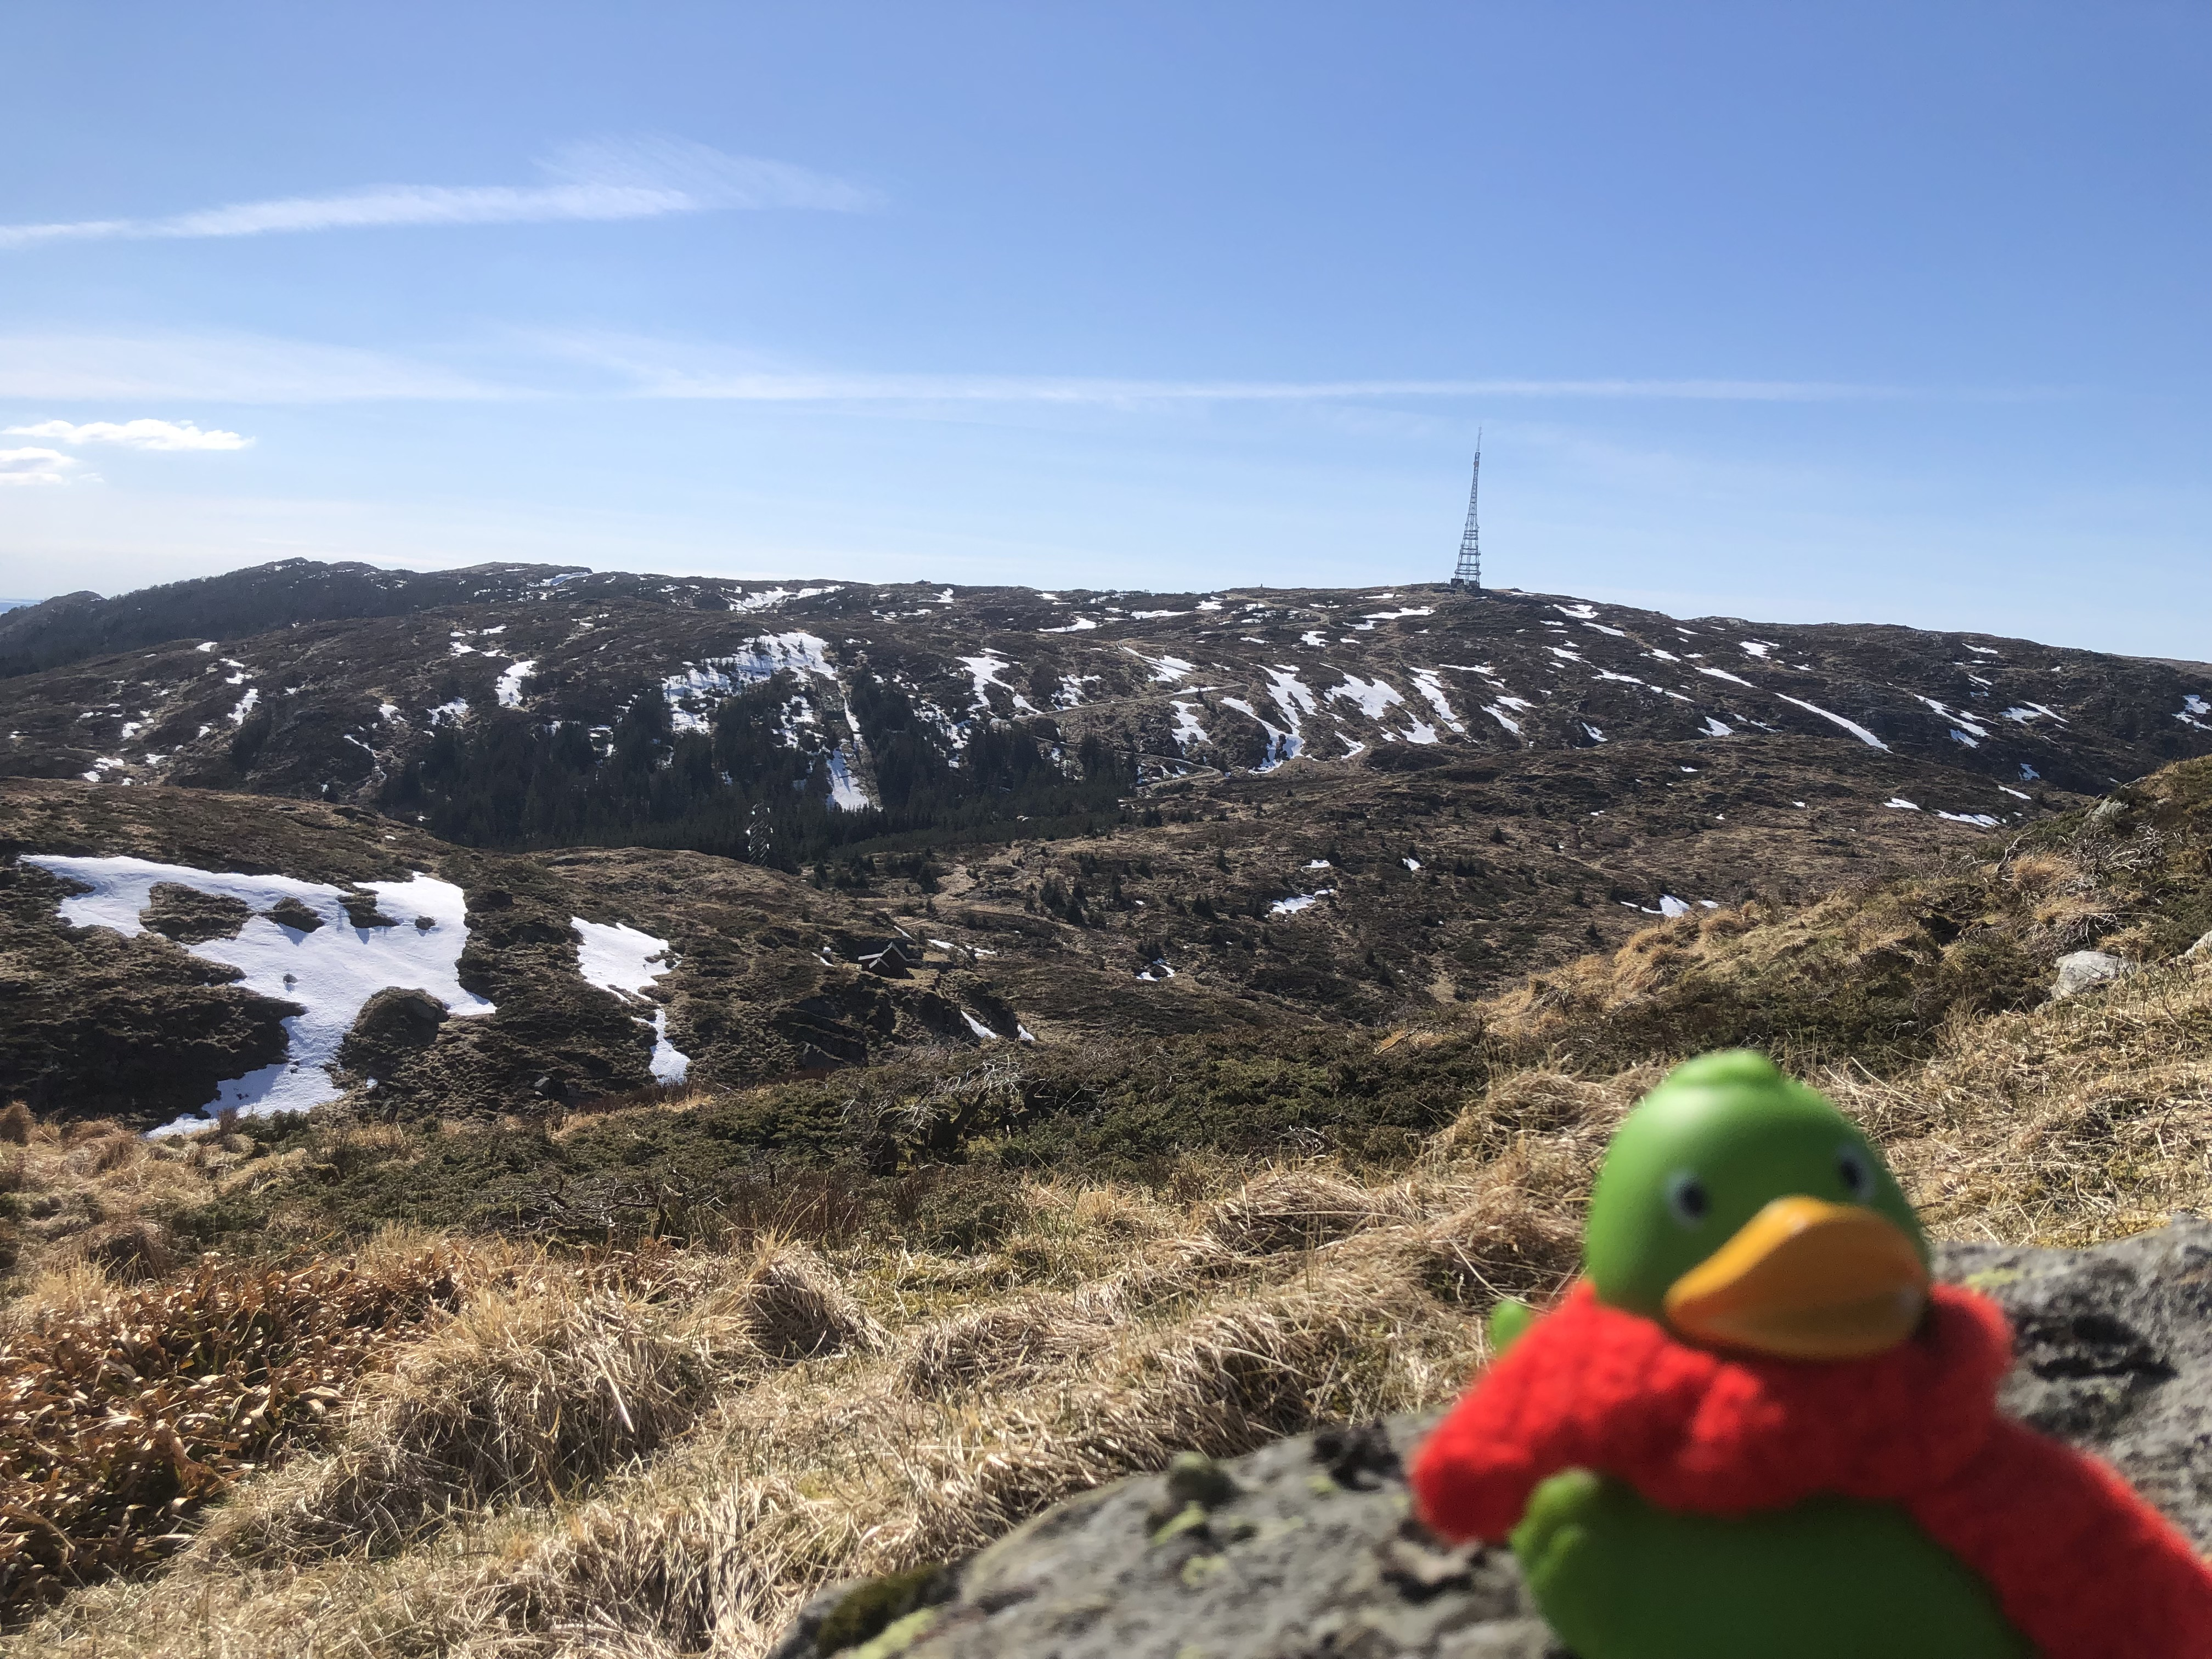
\includegraphics[height = 4.9cm]{guillaume5.jpg}
    \end{figure}
\end{frame}
    \newpage

    \chapter{Signatures}
So far we've defined all our operations as part of our AST. 
By introducing signatures into our compilers we can abstract away the implementation of our operations from the AST.
This allows us to change the implementation of our operations without changing the AST.
Before we can do this we need to talk a bit about the theory behind signatures and algebras

\section{A little bit of Theory}

\subsection{Signatures}
\gls{signature}s are a way to define a set of operations and their types.

Formaly a signature\footnote{also called an \textit{Interface}} is defined as $I = \langle S,F \rangle$ where
\begin{itemize}
    \item $S$ is a set of sorts(aka typenames), and
    \item $F$ is a set of function declarations $f: s_1, ..., s_n \rightarrow s$, for $s1, \dots, s_n, s \in S$
\end{itemize}
Signatures alone do not define any semantics, they are just a way to define which operations and types exist, but not what they do.
To define the semantics we need to define what we call an algebra.

Here's an example of a signature.
\begin{align*}
    Nat = \langle \{&N\},\\ 
                  \{&zero: N,\\
                    &succ: N \rightarrow N\} \rangle
\end{align*}

\subsection{Algebras}
An \gls{algebra} is a way to define the semantics of a signature.
An algebra assigns every sort to a domain and every function to a function on the domains.
An algebra $A$ for a signature $I = \rangle S,F \langle$ defines
\begin{itemize}
    \item a set $[\![s]\!]_A$ for every sort $s \in S$, and
    \item a total function $[\![f]\!]_A : [\![s_1]\!]_A \times ... \times [\![s_k]\!]_A \rightarrow [\![s]\!]_A$ for every  $(f: s_1, ... , s_k \rightarrow s) \in F$
\end{itemize}
It's possible to have multiple algebras for a signature.
Here are a couple of algebras for the $Nat$ signature.

\begin{align*}
    \alg{N}{A_1} &= \mathcal{N}\\
    \alg{zero}{A_1} &= 0\\
    \alg{succ}{A_1} &= \lambda n \mapsto n + 1\\
    &{}\\
    \alg{N}{A_2} &= \{1,2,7\}\\
    \alg{zero}{A_2} &= 2\\
    \alg{succ}{A_2} &= \lambda n \mapsto 7\\
\end{align*}



\section{Implementing Algebraic Specifications}
Integrating signatures and algebras into our interpreter means we can use Algebraic specification theory to formalize and reason about it.
It also lets us change the implementation of our operations without changing the AST and is one step towards user-defined types, and generic programming.

Lets take a look at how we can rewrite an interpreter to make use of signatures.

\begin{figure}[H]
    \lstinputlisting[language=Haskell, firstline=4]{figures/code/signatures/ex1/AST.hs}
    \label{fig:astx}
    \caption{Interpreter for a simple language}
\end{figure}

We do this by creating a new AST without any operations apart from Literals, Variables, and Function calls.
And instead of returning a \texttt{Int} we make it so that the AST can work for any \texttt{valuedomain}(FIgure \ref{fig:ast2}).

\begin{figure}[H]
    \lstinputlisting[language=Haskell, firstline=4, lastline=8]{figures/code/signatures/ex1/AST2.hs}
    \label{fig:ast2}
\end{figure}

We also change the evaluator to reflect this change. One major change(apart from the lack of operations) is that we now need to pass the algebra(\texttt{funmod}) to the evaluator.

\begin{figure}[H]
    \lstinputlisting[language=Haskell, firstline=11]{figures/code/signatures/ex1/AST2.hs}
    \label{fig:eval}
\end{figure}

Not that we've adapted the AST for signatures it's time to implement a signature for the operations we removed.

\begin{figure}[H]
    \lstinputlisting[language=Haskell, firstline=10, lastline=17]{figures/code/signatures/ex1/Intrinsics.hs}
    \label{fig:sig}
\end{figure}
You may have noticed one major change from the old AST. The old AST only worked on \texttt{Int}s, but we've added a second sort \texttt{Bool} to the signature.
Since Haskell only lets us use one type for the valuedomain we need to create a new type that can hold both \texttt{Int}s and \texttt{Bool}s.

\begin{figure}[H]
    \lstinputlisting[language=Haskell, firstline=20, lastline=20]{figures/code/signatures/ex1/Intrinsics.hs}
    \label{fig:valuedomain}
\end{figure}
\newpage

We then define our algebra for the functions in the signature.

\begin{figure}[H]
    \lstinputlisting[language=Haskell, firstline=22]{figures/code/signatures/ex1/Intrinsics.hs}
    \label{fig:alg}
\end{figure}

Now, there are some downsides to using signatures. For one we no longer get to use Haskell's built-in type system to check that we're using the right types.
That means that we need to implement and adapt our type checker to work with signatures.

\subsection{ADTs}
We've implemented Signatures in our interpreter, but we haven't given the user a way to define their own yet. 
We can do this by introducing \gls{adt} in our language.
Abstract Data Types are a way to define a type and its operations without exposing the implementation. \\
The best example of ADTs are probably Interfaces in Java.

Methods in Java Interfaces don't have any implementation\footnote{We'll conveniently ignore the existence of the \texttt{defaul} keyword.}, they just define the signature of the method.
This means that we can define a method in an interface and then implement it in multiple ways.
This is a very powerful tool for generic programming.

\begin{figure}[H]
    \lstinputlisting[language=Java, firstline=1]{figures/code/signatures/ADT/IStack.java}
    \label{fig:istack}
    \caption{ADT for a Stack}
\end{figure}

\newpage

Figure \ref{fig:stack} shows one implementation of \texttt{IStack}.

\begin{figure}[h]
    \lstinputlisting[language=Java, firstline=8, lastline=26]{figures/code/signatures/ADT/Stack.java}
    \label{fig:stack}
    \caption{Stack}
\end{figure}

Since ADTs don't specify an implementation it is perfectly valid for me to implement whatever I want as long as it has the same signature.
For example, I could implement \texttt{IStack} as a linked list instead of an array.
Or we could go a step further and observe that the only difference between stacks and queues is the behavior of \texttt{pop}.\\
So Figure \ref{fig:queue} is a totally valid implementation of the \texttt{Stack} ADT.

\begin{figure}[!h]
    \lstinputlisting[language=Java, firstline=7, lastline=26]{figures/code/signatures/ADT/Queue.java}
    \label{fig:queue}
    \caption{Queue}
\end{figure}
\section{Generic Programming}

\subsection{Concepts}
    \newpage

    %\chapter{MDCS}
    %\newpage

    \appendix

    \chapter{Assertions}
Assertions are a statement that checks that some predicate holds.\\
Assertions ensure that a program is always in a valid state.
If for any reason an assertion fails a program crash is the result.
This is usually the preferred option since an invalid state means that the program behaviour is undefined, and can result in security or safety issues.

\section{Types of Assertions}
\subsection*{Pre-Conditions}
Pre-conditions are assertions that must hold before a function or procedure is called.
They are used to ensure that the function is called with valid arguments and that the function can be executed correctly.

\subsubsection*{Post-Conditions}
Post-conditions are assertions that must hold after a function or procedure is called.
They are used to ensure that the function has been executed correctly and that the result is valid.

\subsection*{Invariants}
Invariants are assertions that must hold at all times.
They are used to ensure that the program is always in a valid state.

For example, we can use assertions to make sure that an implementation of the natural numbers is valid.
We could do this by always checking that any argument, value, or result is always greater than or equal to zero.
    \newpage

    \chapter{Language Standards}

\section{Software Engineering Implications of Languages}
The choice of language can have a massive impact on software development. The move to higher abstraction languages has caused a corresponding increase in efficiency
since the developer can focus all their efforts on what the program should accomplish instead of having to work on the details. 
\gls{SLE} has many applications within software engineering like;

\begin{itemize}
    \item Design, implementation, and usage of DSLs that are tailor-made for a specific problem or technical domains, like, UI, web services, configurations, testing,
            data exchange, interoperability, deployment, and distribution.
    \item Software reverse engineering and re-engineering in many forms, for example, analysis of projects regarding their dependence on open source software,
            integration of systems, and migration of systems constrained by legislation or technology.
    \item Data extraction in the context of data mining, information retrieval, machine learning, big data analytics, social science, digital forensics, and AI, 
            with diverse input, and artifacts to be parsed in interchange formats to conform to.
\end{itemize}

Software languages can also impact the security of any product. If a language has a fundamental flaw or creates unknown pitfalls that might be hard to spot due to
the inherent design of the language could then be exploited by malicious actors. 

\section{Reading spesifications}
\subsection{Backus-Naur Form}
    \gls{BNF} is a format for describing context-free grammar. We use it to describe the syntax of languages. Although it is probably not part of the curriculum
    it's still important to know since most language specification describes their languages using some variation of BNF most common of which is the Extended Backus-Naur form(EBNF).
    An EBNF consists of terminal symbols and non-terminal production rules which are the restrictions governing how terminal symbols can be combined into a legal sequence. 
    Examples of terminal symbols include alphanumeric characters, punctuation marks, and whitespace characters. These constructions often end up looking like Haskell data structures,
    this should hopefully help you understand them.
    \begin{lstlisting}[language=XML]
<symbol> ::= __expression__
    \end{lstlisting}
    Here is the complete PASCAL-like language that only allows assignments. in its EBNF form.
    \begin{lstlisting}[language=XML]
(* a simple program syntax in EBNF - Wikipedia *)
program = 'PROGRAM', white space, identifier, white space, 
    'BEGIN', white space, 
    { assignment, ";", white space }, 
    'END.' ;
identifier = alphabetic character, { alphabetic character | digit } ;
number = [ "-" ], digit, { digit } ;
string = '"' , { all characters - '"' }, '"' ;
assignment = identifier , ":=" , ( number | identifier | string ) ;
alphabetic character = "A" | "B" | "C" | "D" | "E" | "F" | "G"
                | "H" | "I" | "J" | "K" | "L" | "M" | "N"
                | "O" | "P" | "Q" | "R" | "S" | "T" | "U"
                | "V" | "W" | "X" | "Y" | "Z" ;
digit = "0" | "1" | "2" | "3" | "4" | "5" | "6" | "7" | "8" | "9" ;
white space = ? white space characters ? ;
all characters = ? all visible characters ? ;
    \end{lstlisting}

    EBNF also includes regex like syntax for expressing repetition(*,+), optionality(?,[]), and alternatives(|).
    If the above looks confusing or unintuitive I wouldn't worry. The syntax of EBNF is fairly intuitive and most standards have fairly little of it at once.

    \newpage

    %\glsaddall
    %\printglossary[title=Glossary,toctitle=Glossary]
    %\printglossaries
    \addcontentsline{toc}{chapter}{Glossary}
    \printnoidxglossaries
    
    \addcontentsline{toc}{chapter}{Bibliography}
    \bibliography{main}
\end{document}